\capitulo{6}{Trabajos relacionados}

En este apartado se van a presentar diferentes alternativas de herramientas ETL que cubrán de manera parcial o total los requisitos de las tareas completadas con el sistema ELK.

\section{PowerBI}
Esta herramienta de análisis de datos desarrollada por \textit{Microsoft} está más enfocada al mundo de los negocios\cite{PowerBI}. Y al igual que el \textit{stack ELK} proporciona distintos complementos para realizar visualizaciones de datos y poder crear informes interactivos de los mismos.

A diferencia de el \textit{stack ELK } usado en este proyecto, \textbf{PowerBI} \ref{fig:powerbi}esta basado en la nube, alojando ahi el almacenamiento de los datos, la preparación de estos y las visualizaciones personalizadas.

Por su facilidad de uso, las distintas integraciones que ofrece con programas como \textit{Excel} o \textit{SQL Server}, y sus númerosas funciones avanzadas, \textbf{PowerBI} se destaca como el programa líder del sector y más utilizado a nivel global dento de la ciencia de los datos.

\begin{figure}
    \centering
    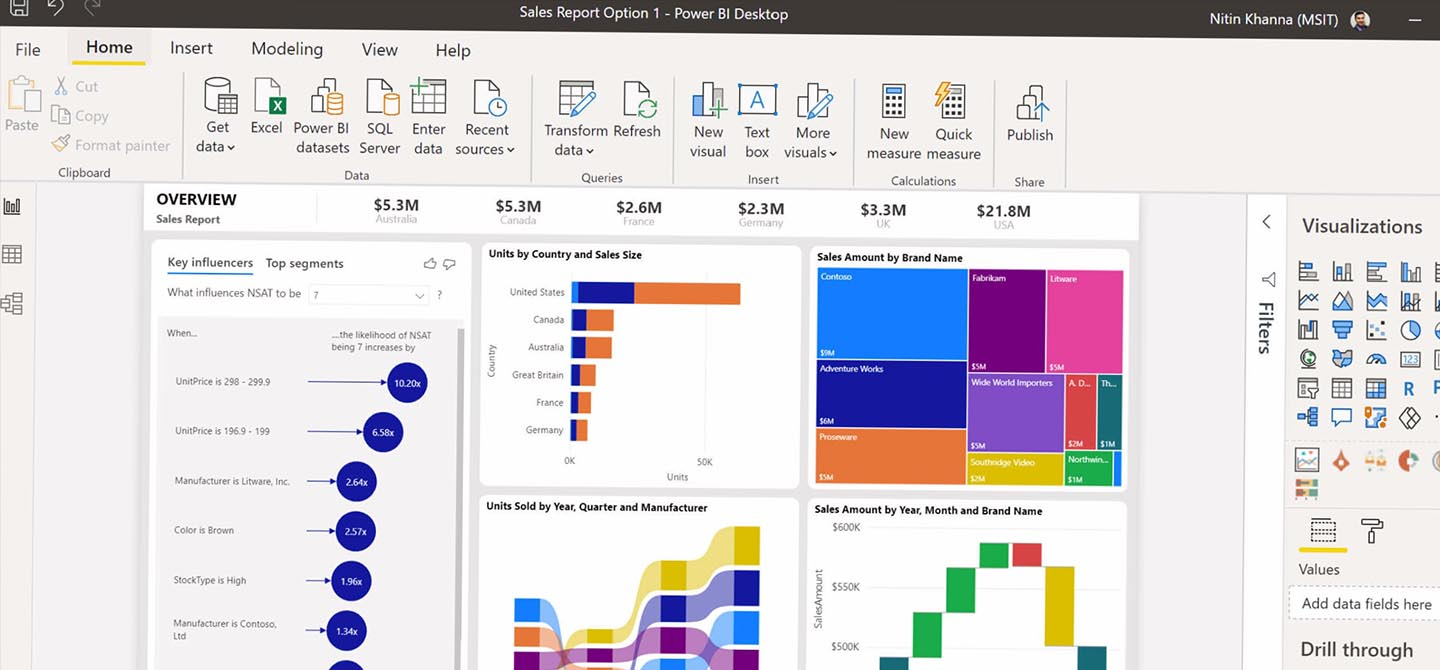
\includegraphics[width=1\linewidth]{img/powerbi.jpg}
    \caption{Visualizaciones de PowerBI \cite{PowerBii}}
    \label{fig:powerbi}
\end{figure}

\paragraph{            }
\paragraph{            }
\paragraph{            }
\paragraph{            }


\section{Spoon y Qlik}
Tuve la oportunidad de realizar las prácticas en la empresa informática CSA (Centro de Servicios Avanzados), concretamente en el departamento de Business Intelligence (BI) y Automatización y Robótica de Procesos (RPA). 

Aquí estuve trabajando con su sistema de herramientas ETL el cuál tenía una estructura diferente pero la finalidad era la misma que la del \textit{Stack ELK}, extraer, transformar y cargar información.

Lo primero era extraer la información de los diferentes servidores y bases de datos de la empresa, y el primer paso para administrar estas bases se hacia a través el programa \textbf{DBeaver}. Una vez teniamos claros los archivos a tratar con la herramienta \textbf{WinSCP} gestionábamos los datos en cuestión. 

La herramienta equivalente a Logstash era \textbf{Spoon} \ref{fig:spoon}, una interfaz para diseñar soluciones de transformación de datos que nos permite crear procesos de carga y lectura de manera intuitiva y visual.

\begin{figure}
    \centering
    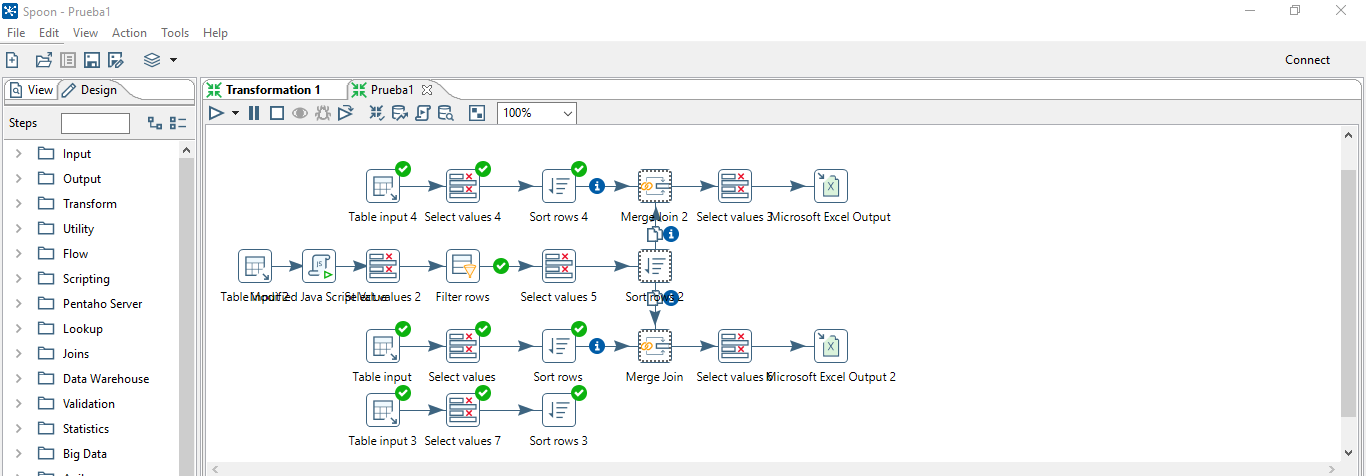
\includegraphics[width=1\linewidth]{img/spoon.png}
    \caption{Estructura de Spoon \cite{Spoon} }
    \label{fig:spoon}
\end{figure}

Y por último, la herramienta estrella, \textbf{Qlik}  \ref{fig:qlik}, que nos permite pintar gráficos e interfaces con todos los datos procesados por las herramientas anteriores.

\begin{figure}
    \centering
    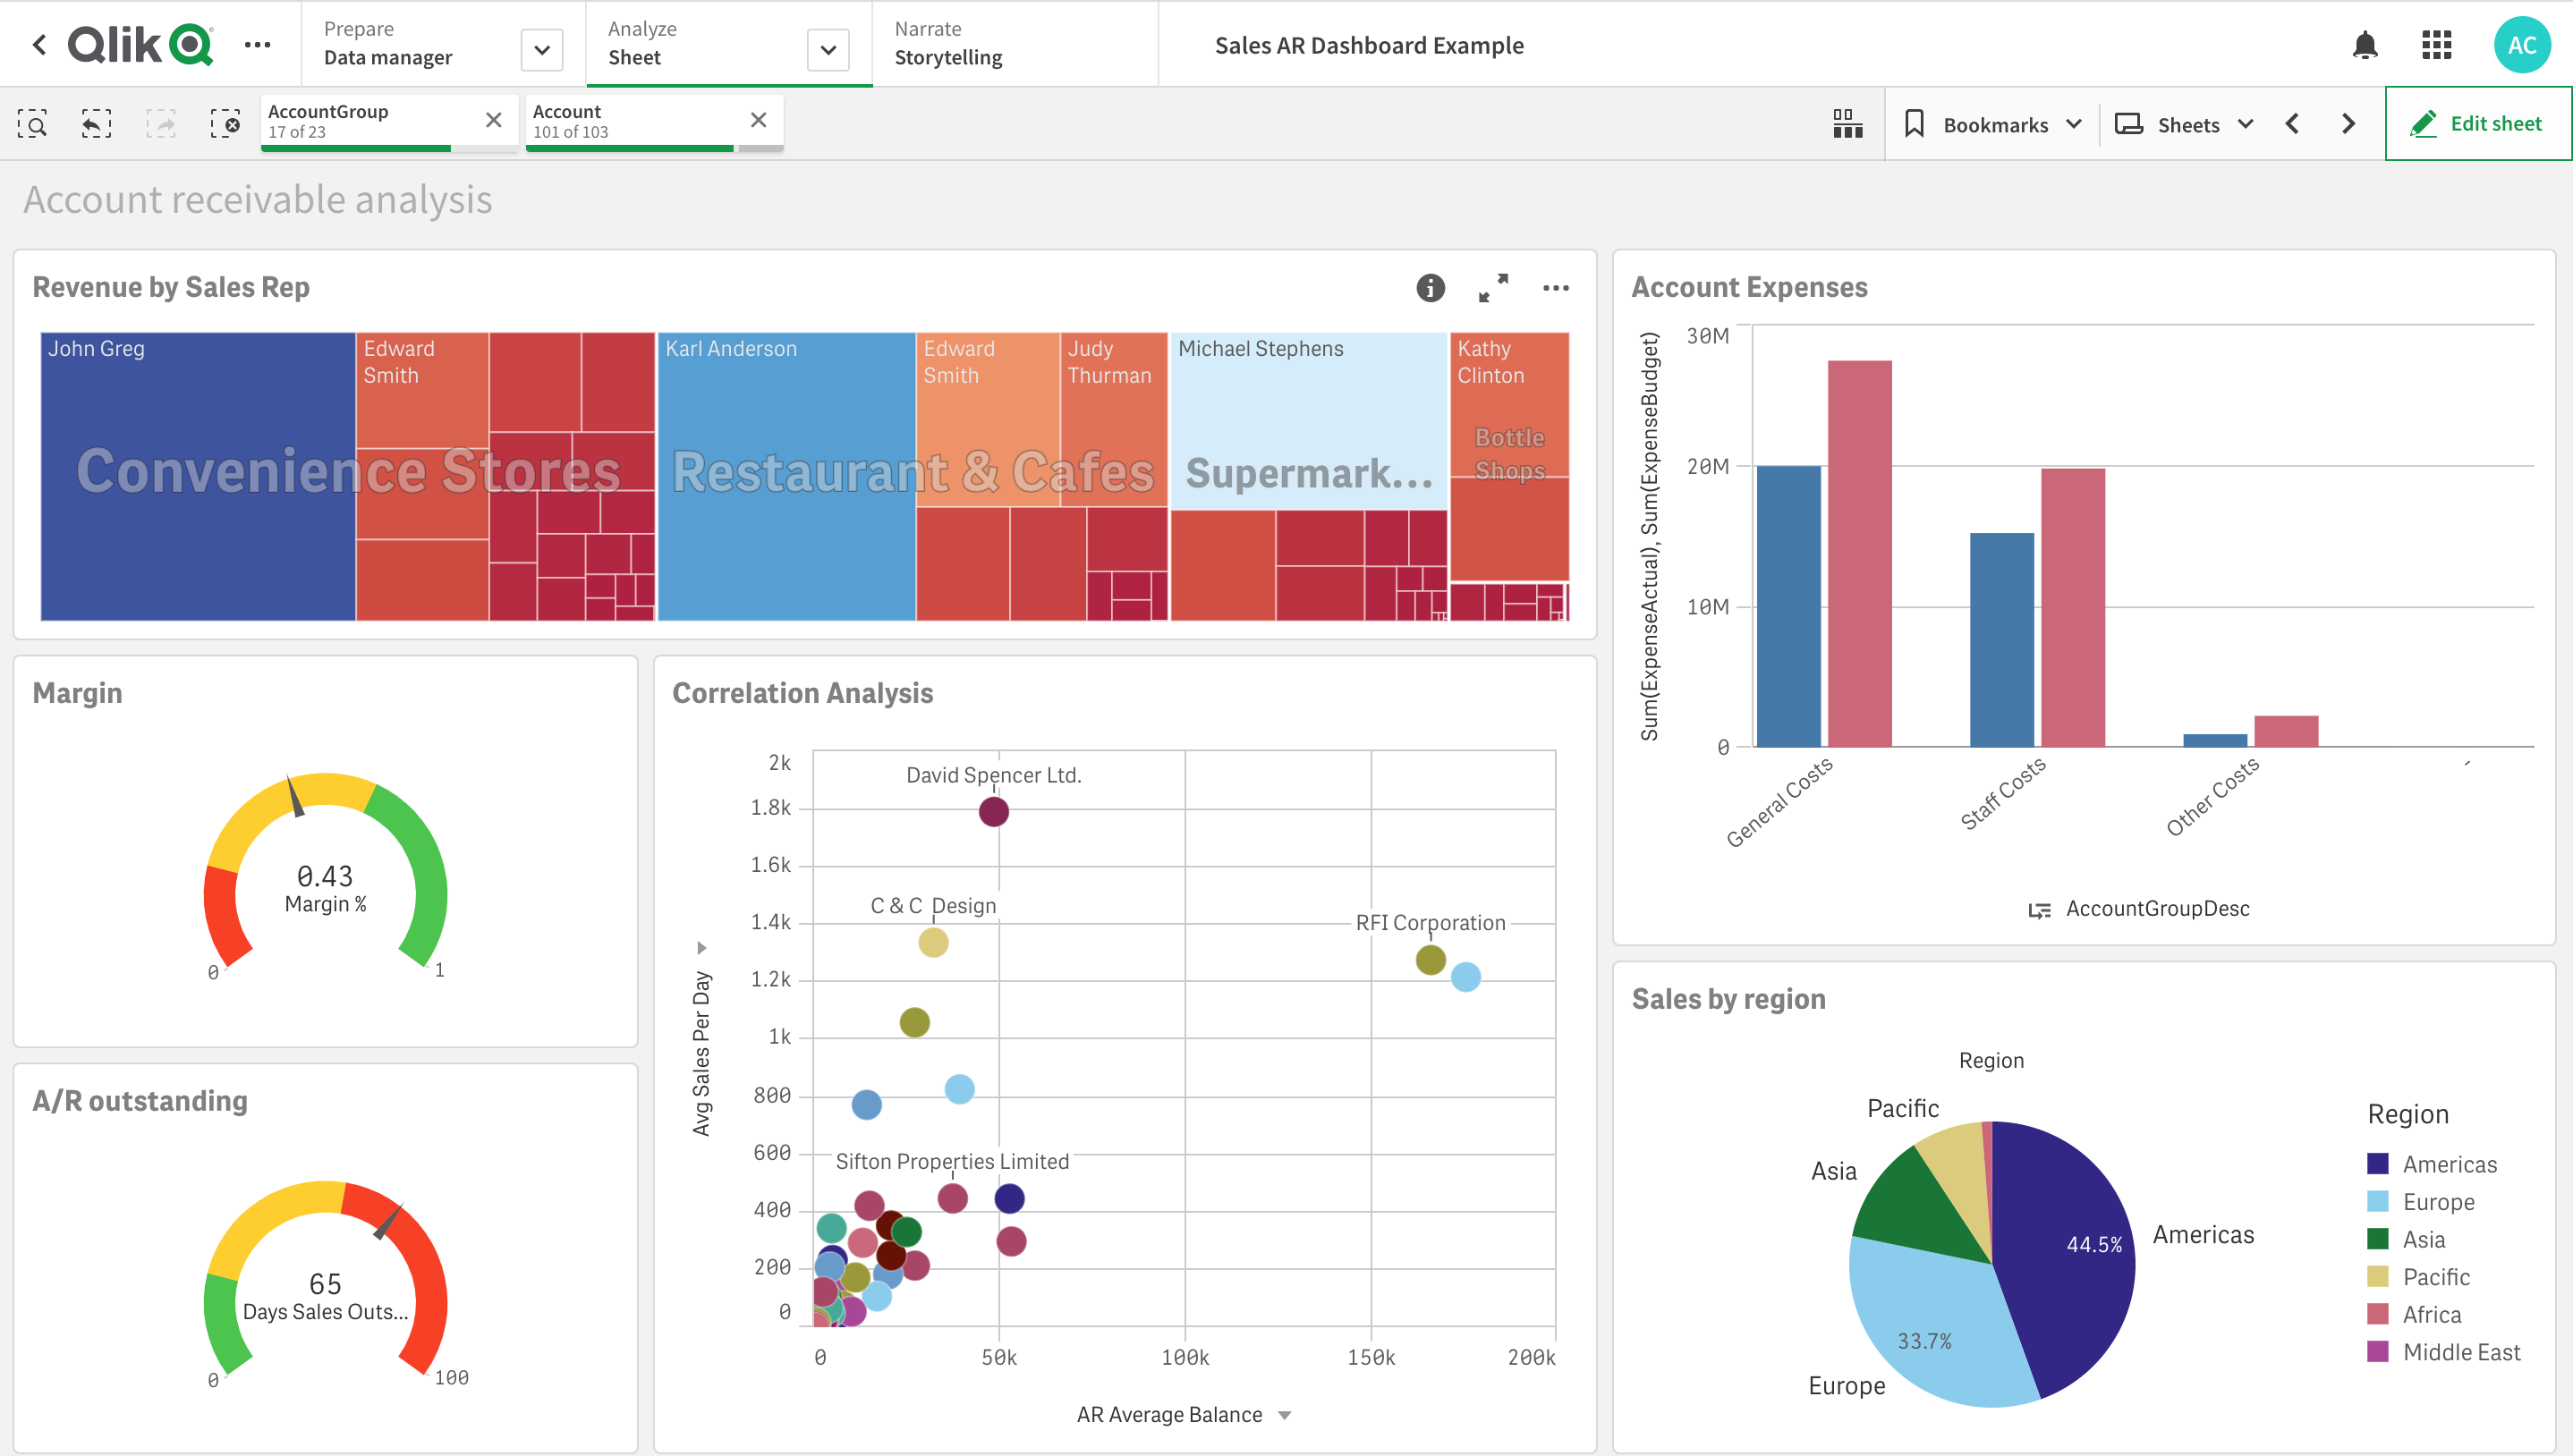
\includegraphics[width=1\linewidth]{img/qlik.png}
    \caption{Visualizciones con Qlik \cite{Qlik} }
    \label{fig:qlik}
\end{figure}

\paragraph{            }
\paragraph{            }

\section{Tableau}
Este software está pensado para el desarrollo de visualizaciones interactivas  de datos en forma de gráficos en \textit{dashboards} \ref{fig:tableau}. Fue diseñado para el análisis y comprensión de datos complejos ya que soporta la ingesta de datos tanto desde hojas de cálculo como de bases de datos. Posee una interfaz intuitiva basada en \textit{drag and drop} de manera que cualquier usuario pueda comprender y tomar decisiones basadas en información de datos.

\begin{figure}
    \centering
    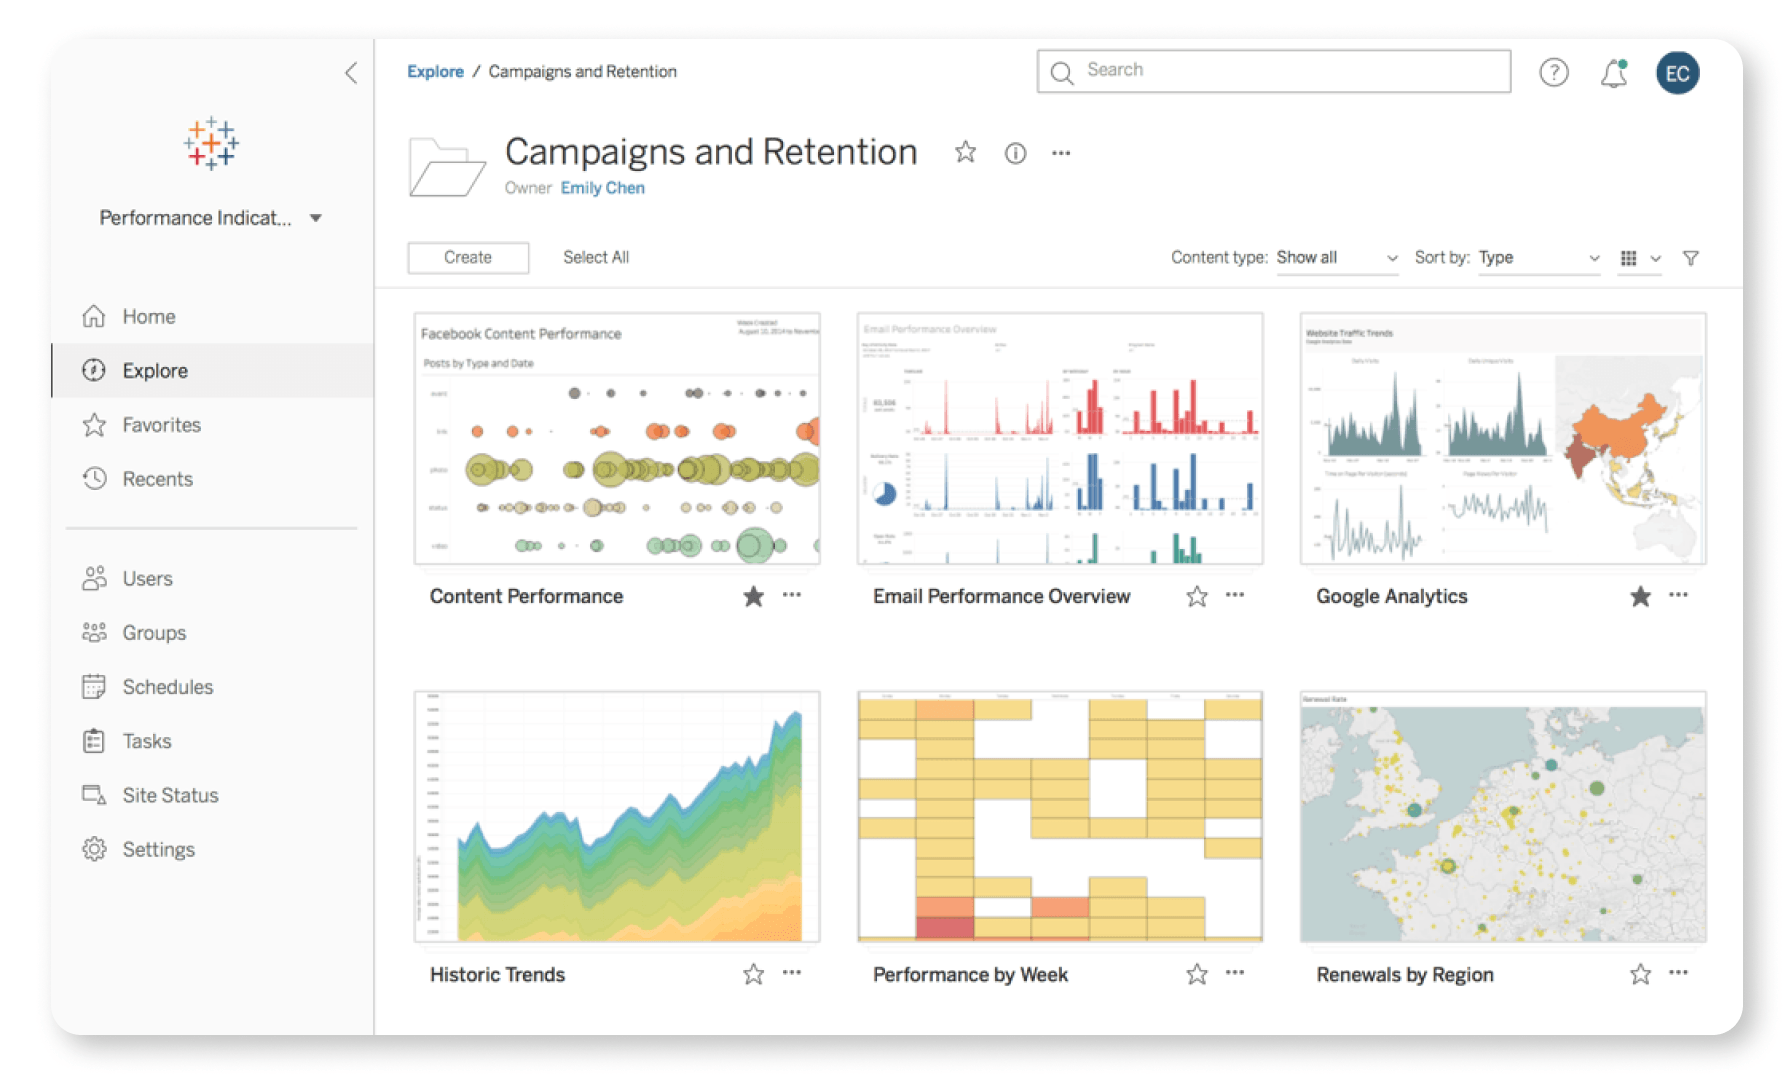
\includegraphics[width=1\linewidth]{img/tableau.png}
    \caption{Dashboard principal de Tableau \cite{tableau}}
    \label{fig:tableau}
\end{figure}
\section{Splunk}
Consiste en una plataforma diseña para analizar y monitorear datos ingestados en tiempo real \ref{fig:splunk}. Este software recopila e indexa grandes conjuntos de datos de manera que se puedan filtrar y analizar de manera profunda y avanzada a la hora de identificar anomalías, optimizar procesos o identificar patrones.

\begin{figure}
    \centering
    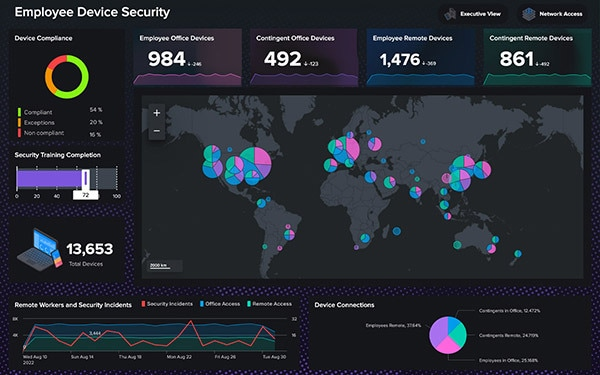
\includegraphics[width=1\linewidth]{img/splunk.jpg}
    \caption{Dashboard básico de Splunk \cite{splunk}}
    \label{fig:splunk}
\end{figure}

\section{Comparativa entre alternativas}

A continuación se realizará una tabla comparativa entre las diferentes opciones expuestas en este apartado como alternativas al stack ELK, así como más opciones presentes en el mercado. Se incluyen algunas características o propiedas que resultan interesantes. \ref{tab:comparacion}

Cabe destacar que las funciones de inteligencia artificial en el caso del stack ELK se considerena limitadas, ya que ofrece detección de anomalías y un plugin para uso de machine learning. Ambas funciones solo están disponibles en el plan de suscripción Platinum, por lo que se consideran escasas en comparación con PowerBI, el cuál integra machine learning para realizar modelos predictivos o analizar series temporales. Qlik, Tableau y Splunk ofrecen características muy similares de este tipo sobre todo enfocadas al análisis y procesamiento de datos en tiempo real.

Como conclusión indicar que el stack ELK está pensado para monitorizar y analizar datos, principalmente de tipo log, en tiempo real, no como PowerBi que está más enfocado al ámbito empresarial a la hora de generar informes (ideal si el ecosistema en el que se trabaja es el de Microsoft). Qlik y Spoon son una buena combinación para negocios basados en ETL, al igual que Tableau y Splunk al ser todas herramientas para usos muy similares.


\begin{table}[h]
\centering
\begin{tabularx}{\textwidth}{|X|X|X|X|X|X|}
\hline
 & \textbf{Stack ELK} & \textbf{Power BI} & \textbf{Qlik + Spoon} & \textbf{Tableau} & \textbf{Splunk} \\ \hline
\textbf{Función principal} & Análisis de logs y datos en tiempo real & Análisis de negocios y generación de informes & Análisis de negocios y ETL & Visualización de datos de negocios & Análisis de datos en tiempo real \\ \hline
\textbf{Facilidad de uso} & Requiere conocimientos técnicos avanzados & Interfaz intuitiva y fácil de usar & Qlik es más intuitivo que Spoon & Interfaz intuitiva y fácil de usar & Requiere conocimientos técnicos avanzados \\ \hline
\textbf{Escalabilidad} & Alta & Limitada & Alta & Alta & Alta \\ \hline
\textbf{Coste} & Gratis, opciones avanzadas de pago & Suscripción de pago & Qlik licencia de pago, Spoon es gratis & Suscripción de pago & Suscripción de pago \\ \hline
\textbf{Almacenamiento en la Nube} & Lo proporciona el servicio de pago Elasticsearch Service & Sí, integrado con Azure & Qlik sí que lo ofrece y Spoon puede integrarse & Sí, integrado con servicios en la nube & Sí, integrado con servicios en la nube \\ \hline
\textbf{Análisis en Tiempo Real} & Sí, nativo & Depende de la fuente de datos & Sí, Qlik permite análisis en tiempo real & Depende de la fuente de datos & Sí, nativo \\ \hline
\textbf{Inteligencia Artificial} & Funcionalidades limitadas & Ofrece capacidades de IA y análisis predictivo & Qlik tiene capacidades de IA, Spoon no & Ofrece IA y análisis predictivo & Ofrece IA y análisis predictivo \\ \hline
\textbf{Sistemas Operativos} & Windows, Linux y Mac & Windows y Mac & Windows, Linux y Mac & Windows, Linux y Mac & Windows, Linux y Mac \\
\end{tabularx}
\caption{Comparación entre herramientas ETL}
\label{tab:comparacion}
\end{table}
